\documentclass{article}
\usepackage[utf8]{inputenc}
% are all of these packages really necessary?
% no.
% i'm just too lazy to only grab the packages i want for a specific
% document, so i just glob all of my most commonly used packages together
% this is bad practice.
\usepackage{amsmath,amsthm,amssymb,amsfonts, fancyhdr, color, comment, graphicx, environ, mdframed, soul, calc, enumitem, mdframed, xcolor, geometry, empheq, mathtools, tikz, pgfplots}

\usetikzlibrary{external}
\tikzexternalize[prefix=tikz/,optimize command away=\includepdf]

%tikzpicture
\usepackage{tikz}
\usepackage{scalerel}
\usepackage{pict2e}
\usepackage{tkz-euclide}
\usetikzlibrary{calc}
\usetikzlibrary{patterns,arrows.meta}
\usetikzlibrary{shadows}
\usetikzlibrary{external}

%pgfplots
\usepackage{pgfplots}
\pgfplotsset{compat=newest}
\usepgfplotslibrary{statistics}
\usepgfplotslibrary{fillbetween}

\tikzset{external/export=true}
\pgfplotsset{
    standard/.style={
    axis line style = thick,
    trig format=rad,
    enlargelimits,
    axis x line=middle,
    axis y line=middle,
    enlarge x limits=0.15,
    enlarge y limits=0.15,
    every axis x label/.style={at={(current axis.right of origin)},anchor=north west},
    every axis y label/.style={at={(current axis.above origin)},anchor=south east}
    }
}
\newcommand*\widefbox[1]{\fbox{\hspace{2em}#1\hspace{2em}}}
% Command "alignedbox{}{}" for a box within an align environment
% Source: http://www.latex-community.org/forum/viewtopic.php?f=46&t=8144
\newlength\dlf  % Define a new measure, dlf
\newcommand\alignedbox[2]{
% Argument #1 = before & if there were no box (lhs)
% Argument #2 = after & if there were no box (rhs)
&  % Alignment sign of the line
{
\settowidth\dlf{$\displaystyle #1$}  
    % The width of \dlf is the width of the lhs, with a displaystyle font
\addtolength\dlf{\fboxsep+\fboxrule}  
    % Add to it the distance to the box, and the width of the line of the box
\hspace{-\dlf}  
    % Move everything dlf units to the left, so that & #1 #2 is aligned under #1 & #2
\boxed{#1 #2}
    % Put a box around lhs and rhs
}
}

\newcommand{\lrp}[1]{\left( #1 \right)}
\newcommand{\abs}[1]{\left\vert #1 \right\vert}
\newcommand{\lra}[1]{\left\langle #1 \right\rangle}
\newcommand{\lrb}[1]{\left[ #1 \right]}
\newcommand{\iintR}[0]{\iint\limits_{R}}

\geometry{letterpaper, portrait, margin=1in}
\renewcommand{\footrulewidth}{0.8pt}
\setlength\parindent{0pt}
\pagestyle{fancy}
\lhead{Christina Phan}
\rhead{MAT 21D} 
\chead{\textbf{Homework 2 Solutions}}

\newcommand{\Solution}{\textit{Solution}}
 \pgfplotsset{compat=1.18}
\begin{document}
\textbf{Problem 1}

Evaluate the integral:

\textbf{(a)} $\displaystyle \int_0^\pi \int_0^x x\sin y\,dy\,dx$

\Solution
\begin{align*}
    \int_0^\pi \int_0^x x\sin y\,dy\,dx&=\int_0^\pi \lrb{-x\cos y}_0^x\,dx\\
    &=\int_0^\pi -x\cos x + x\,dx\\
    &=\int_0^\pi -x\cos x \,dx+\int_0^\pi x \,dx\\
    &u=-x\hspace{2em}dv=\cos x\,dx\\
    &du=-dx\hspace{2em}v=\sin x\\
    &=\lrb{-x\sin x}_0^\pi +\int_0^\pi \sin x\,dx + \lrb{\frac{1}{2}x^2}_0^\pi\\
    &=\lrp{0-0}+\lrb{-\cos x x}_0^\pi + \lrp{\frac{1}{2}\pi^2-0}\\
    &=(0-0)+(1+1)+\frac{1}{2}\pi^2\\
    &=\boxed{2+\frac{1}{2}\pi^2}
\end{align*}
\textbf{(b)} $\displaystyle \int_0^1\int_0^{y^2}3y^3e^{xy}\,dx\,dy$

\Solution
\begin{align*}
    \int_0^1\int_0^{y^2}3y^3e^{xy}\,dx\,dy&=\int_0^1\lrb{3y^2e^{xy}}_0^{y^2}\,dy\\
    &=\int_0^1 3y^2e^{y^3}-3y^2\,dy\\
    &=\lrb{e^{y^3}-y^3}_0^1\tag{you could also u-sub...}\\
    &=\lrp{e-1}-\lrp{1-0}\\
    &=\boxed{e-2}
\end{align*}

\textbf{Problem 2}

Integrate the function $\displaystyle f(x,y)=\frac{x}{y}$ over the quadrilateral in the first quadrant bounded by the lines $y=x$, $y=2x$, $x=1$, and $x=2$.

\Solution

It may be helpful to graph the lines to see which functions go on the top/bottom, left/right.
Remember: constants go on the outside!
\begin{align*}
    \iint_R \frac{x}{y}\,dA&=\int_1^2\int_x^{2x} \frac{x}{y}\,dy\,dx\\
    &=\int_1^2\lrb{x\ln\left|y\right|}_x^{2x}\,dx\\
    &=\int_1^2 x\ln (2x) - x\ln (x) \,dx\tag{ok to drop abs since always positive}\\
    &=\int_1^2 x\big(\ln (2x)-\ln (x)\big)\,dx\\
    &=\int_1^2 x\lrp{\ln \frac{2x}{x}}\,dx\tag{properties of log}\\
    &=\int_1^2 x(\ln 2)\,dx\\
    &=\lrb{\frac{\ln 2}{2}x^2}_1^2\\
    &=2\ln 2 - \frac{1}{2}\ln 2\\
    &=\boxed{\frac{3}{2}\ln 2}
\end{align*}
\textbf{Problem 3}

Write an equivalent double integral with the order of integration reversed (you may find it helpful to sketch the region of integration):

\textbf{(a)} $\displaystyle \int_0^2\int_{y-2}^0\,dx\,dy$

\Solution

Let's sketch the region. That is, graph $y=0$, $y=2$, $x=y-2$ and $x=0$.
\begin{center}
\resizebox{3.5cm}{!}{
    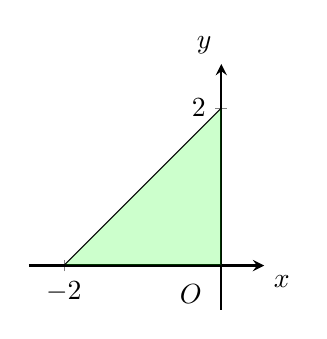
\begin{tikzpicture}
    \begin{axis}[standard,
            xtick={-2},
            ytick={2},
            samples=1000,
            xlabel={$x$},
            ylabel={$y$},
            xmin=-2.1,xmax=0.2,
            ymin=-0.2,ymax=2.2,
            x=1cm,
            y=1cm/1,
           ]
\node[anchor=center,label=south west:$O$] at (axis cs:0,0){};
\addplot[name path=F,domain={-2:0}]{x+2};
\addplot[name path=y2, domain={-2:0}]coordinates{(-2,0) (0,0)};
\addplot[fill=green, fill opacity=0.2] fill between [of=F and y2, soft clip={domain=-2:0}];
    \end{axis}
    \end{tikzpicture}
}
\end{center}
When we reverse the order of integration, we'll have $x$ be on the outside.

The lowest $x$ will be is $-2$ and the highest $x$ will be is $0$. Therefore, our boundary for $x$ is $-2\leq x \leq 0$.

For $y$, the lowest $y$ will be (in terms of $x$) is $y=0x=0$ and the highest $y$ will be is $y=x+2$. Therefore, our boundary for $y$ is $0\leq y \leq x+2$.

Putting this all together, we get
\begin{equation*}
\boxed{\int_0^2\int_{y-2}^0\,dx\,dy=\int_{-2}^0\int_0^{x+2}\,dy\,dx}
\end{equation*}
\textbf{(b)} $\displaystyle \int_0^1\int_{1-x}^{1-x^2}\,dy\,dx$

\Solution

Let's sketch the region. That is, graph $x=0$, $x=1$, $y=1-x$, and $y=1-x^2$.
\begin{center}
\resizebox{3.5cm}{!}{
    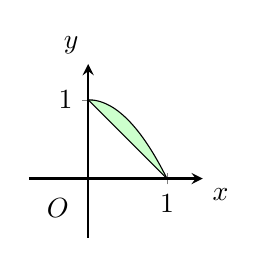
\begin{tikzpicture}
    \begin{axis}[standard,
            xtick={1},
            ytick={1},
            samples=1000,
            xlabel={$x$},
            ylabel={$y$},
            xmin=-0.5,xmax=1.2,
            ymin=-0.5,ymax=1.2,
            x=1cm,
            y=1cm/1,
           ]
\node[anchor=center,label=south west:$O$] at (axis cs:0,0){};
\addplot[name path=F,domain={0:1}]{1-x^2};
\addplot[name path=G,domain={0:1}]{1-x};
\addplot[fill=green, fill opacity=0.2] fill between [of=F and G, soft clip={domain=0:1}];
    \end{axis}
    \end{tikzpicture}
}
\end{center}
When we reverse the order of integration, we'll have $y$ be on the outside.

The lowest $y$ will be is $0$ and the highest $y$ will be is $1$. Therefore, our boundary for $y$ is $0\leq y\leq 1$.

For $x$, the lowest $x$ will be (in terms of $y$) is $x=1-y$ and the highest $x$ will be is $x=\sqrt{1-y}$. Therefore, our boundary for $x$ is $1-y\leq x \leq \sqrt{1-y}$.

Putting this all together, we get
\begin{equation*}
    \boxed{\int_0^1\int_{1-x}^{1-x^2}\,dy\,dx=\int_0^1\int_{1-y}^{\sqrt{1-y}}\,dx\,dy}
\end{equation*}
\textbf{(c)} $\displaystyle \int_0^{\ln 2}\int_{e^y}^2\,dx\,dy$

\Solution

Let's sketch the region. That is, graph $y=0$, $y=\ln 2$, $x=e^y$ and $x=2$.
\begin{center}
\resizebox{3.5cm}{!}{
    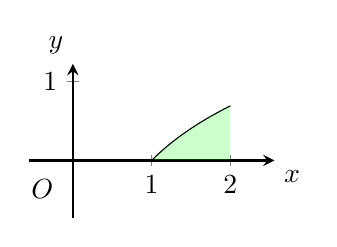
\begin{tikzpicture}
    \begin{axis}[standard,
            xtick={1,2},
            ytick={1},
            samples=1000,
            xlabel={$x$},
            ylabel={$y$},
            xmin=-0.2,xmax=2.2,
            ymin=-0.5,ymax=1,
            x=1cm,
            y=1cm/1,
           ]
\node[anchor=center,label=south west:$O$] at (axis cs:0,0){};
\addplot[name path=F,domain={1:2}]{ln(x)};
\addplot[name path=y2, domain={1:2}]coordinates{(1,0) (2,0)};
\addplot[fill=green, fill opacity=0.2] fill between [of=F and y2, soft clip={domain=1:2}];
    \end{axis}
    \end{tikzpicture}
}
\end{center}
When we reverse the order of integration, we'll have $x$ be on the outside.

The lowest $x$ will be is $1$ and the highest $x$ will be is $2$. Therefore, our boundary for $x$ is $1\leq x\leq 2$.

For $y$, the lowest $y$ will be (in terms of $x$) is $y=0x=0$ and the highest $y$ will be is $y=\ln x$. Therefore, our boundary for $y$ is $0\leq y \leq \ln x$.

Putting this all together, we get
\begin{equation*}
    \boxed{\int_0^{\ln 2}\int_{e^y}^2\,dx\,dy=\int_1^2\int_0^{\ln x}\,dy\,dx}
\end{equation*}
\textbf{(d)} $\displaystyle \int_0^{\pi / 6}\int_{\sin x}^{1/2}xy^2\,dy\,dx$

\Solution

Let's sketch the region. That is, graph $x=0$, $x=\pi/6$, $y=\sin x$, and $y=1/2$
\begin{center}
\resizebox{3.5cm}{!}{
    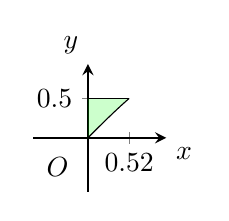
\begin{tikzpicture}
    \begin{axis}[standard,
            xtick={0.5235},
            ytick={0.5},
            samples=1000,
            xlabel={$x$},
            ylabel={$y$},
            xmin=-0.5,xmax=0.8,
            ymin=-0.5,ymax=0.75,
            x=1cm,
            y=1cm/1,
           ]
\node[anchor=center,label=south west:$O$] at (axis cs:0,0){};
\addplot[name path=F,domain={0:0.5235}]{sin(x)};
\addplot[name path=y2, domain={0:0.5235}]coordinates{(0,0.5) (0.5235,0.5)};
\addplot[fill=green, fill opacity=0.2] fill between [of=F and y2, soft clip={domain=0:0.5235}];
    \end{axis}
    \end{tikzpicture}
}
\end{center}
Yes, that looks like a straight line, but I swear that's supposed to be $y=\sin x$.

When we reverse the order of integration, we'll have $y$ be on the outside.

The lowest $y$ will be is $0$ and the highest $y$ will be is $1/2$. Therefore, our boundary for $y$ is $0\leq y\leq 1/2$.

For $x$, the lowest $x$ will be (in terms of $y$) is $x=0y=0$ and the highest $x$ will be is $x=\sin^{-1} y$. Therefore, our boundary for $x$ is $0\leq x \leq \sin^{-1} y$.

Putting it all together, we get
\begin{equation*}
    \boxed{\int_0^{\pi / 6}\int_{\sin x}^{1/2}xy^2\,dy\,dx=\int_0^{\frac{1}{2}}\int_0^{\sin^{-1}y}xy^2\,dx\,dy}
\end{equation*}
\textbf{Problem 4}

Reverse the order of integration and evaluate the integral.

\textbf{(a)} $\displaystyle \int_0^2\int_x^2 2y^2\sin xy\,dy\,dx$

\Solution

It's a good idea to graph the boundaries. That is, graph $x=0$, $x=2$, $y=x$ and $y=2$.

\begin{center}
\resizebox{3.5cm}{!}{
    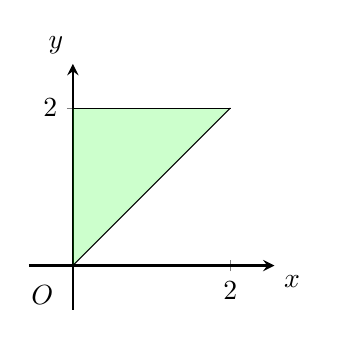
\begin{tikzpicture}
    \begin{axis}[standard,
            xtick={2},
            ytick={2},
            samples=1000,
            xlabel={$x$},
            ylabel={$y$},
            xmin=-0.2,xmax=2.2,
            ymin=-0.2,ymax=2.2,
            x=1cm,
            y=1cm/1,
           ]
\node[anchor=center,label=south west:$O$] at (axis cs:0,0){};
\addplot[name path=F,domain={0:2}]{x};
\addplot[name path=G, domain={0:2}]{2};
\addplot[fill=green, fill opacity=0.2] fill between [of=F and G, soft clip={domain=0:2}];
    \end{axis}
    \end{tikzpicture}
}
\end{center}
If we want to reverse the order of integration, we'll need to have $y$'s on the outside. This means that we need $y=c$'s where $c$ is a constant.

Based on our graph, that would mean $y=0$ and $y=2$ (the lowest $y$ gets is $0$ and the highest $y$ gets is $2$).

For our $x$'s, we need to think in terms of left-to-right. That is, our left line would be $x=0$ and our right line would be $x=y$.

Putting this all together, we get
\begin{align*}
    \int_0^2\int_x^2 2y^2\sin xy\,dy\,dx&=\int_0^2\int_0^y 2y^2\sin xy \,dx\,dy\\
    &=\int_0^2\lrb{-2y\cos xy}_0^y\,dy\\
    &=\int_0^2 -2y\cos y^2 + 2y\,dy\\
    &=-\int_0^2 2y\cos y^2\,dy + \int_0^2 2y\,dy\\
    &u=y^2\hspace{2em}du=2y\,dy\\
    &u(0)=0\hspace{2em}u(2)=4\\
    &=-\int_0^4 \cos u\,du+\lrb{y^2}_0^2\\
    &=-\lrb{\sin u}_0^4 + (4-0)\\
    &=\boxed{-\sin 4 + 4}
\end{align*}
\textbf{(b)} $\displaystyle \int_0^2\int_0^{4-x^2}\frac{xe^{2y}}{4-y}\,dy\,dx$

\Solution

It's a good idea to graph the boundaries. That is, graph $x=0$, $x=2$, $y=0$, and $y=4-x^2$
\begin{center}
\resizebox{3.5cm}{!}{
    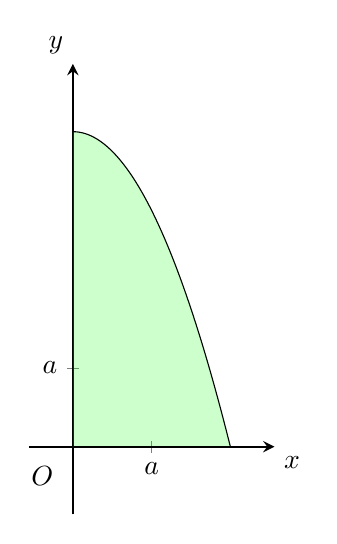
\begin{tikzpicture}
    \begin{axis}[standard,
            xtick={-1, 1},
            ytick={-1, 1},
            samples=1000,
            xlabel={$x$},
            ylabel={$y$},
            xmin=-0.2,xmax=2.2,
            ymin=-0.2,ymax=4.2,
            x=1cm,
            y=1cm/1,
            xticklabels={$-a$, $a$},
            yticklabels={$-a$, $a$}
           ]
\node[anchor=center,label=south west:$O$] at (axis cs:0,0){};
\addplot[name path=F,domain={0:2}]{4-x^2};
\addplot[name path=G, domain={0:2}]{0};
\addplot[fill=green, fill opacity=0.2] fill between [of=F and G, soft clip={domain=0:2}];
    \end{axis}
    \end{tikzpicture}
}
\end{center}

If we reverse the order of integration, we would have the $y$'s on the outside. 
Based on our graph, $0\leq y \leq 4$.

For the $x$'s, in terms of $y$, $0\leq x \leq \sqrt{4-y}$.

Putting this all together, we get
\begin{align*}
    \int_0^2\int_0^{4-x^2}\frac{xe^{2y}}{4-y}\,dy\,dx&=\int_0^4\int_0^{\sqrt{4-y}}\frac{xe^{2y}}{4-y}\,dx\,dy\\
    &=\int_0^4\lrb{\frac{x^2e^{2y}}{2(4-y)}}_0^{\sqrt{4-y}}\,dy\\
    &=\int_0^4\frac{(4-y)e^{2y}}{2(4-y)}\,dy\\
    &=\int_0^4\frac{e^{2y}}{2}\,dy\tag{ok to ``cancel"}\\
    &=\lrb{\frac{e^{2y}}{4}}_0^4\\
    &=\boxed{\frac{e^8}{4}-\frac{1}{4}}
    \end{align*}
\textbf{(c)} $\displaystyle \int_0^8\int_{\sqrt[3]{x}}^2\frac{1}{y^4+1}\,dy\,dx$

\Solution

It's a good idea to graph the boundaries. That is, graph $x=0$, $x=8$, $y=\sqrt[3]{x}$, and $y=2$.

\textit{this graph isn't playing nice with my \LaTeX set up, so desmos is your friend :)}

If we reverse the order of integration, we would have the $y$'s equal constants. Based on our graph, that would mean $y=0$ and $y=2$. 

For our $x$'s, we would get $x=0$ and $x=y^3$.

Putting this all together, we get
\begin{align*}
    \int_0^8\int_{\sqrt[3]{x}}^2\frac{1}{y^4+1}\,dy\,dx&=\int_0^2\int_0^{y^3}\frac{1}{y^4+1}\,dx\,dy\\
    &=\int_0^2\lrb{\frac{1}{y^4+1}x}_0^{y^3}\,dy\\
    &=\int_0^2 \frac{y^3}{y^4+1}\,dy\\
    &=\lrb{\frac{1}{4}\ln\left|y^4+1\right|}_0^2\tag{u-sub with $u=y^4$}\\
    &=\boxed{\frac{1}{4}\ln 17}
\end{align*}

\textbf{(d)} $\displaystyle \int_0^{1/16}\int_{y^{1/4}}^{1/2}\cos 16\pi x^5\,dx\,dy$

\Solution

It's a good idea to graph the boundaries. That is, graph $y=0$, $y=1/16$, $x=y^{1/4}$, $x=1/2$.

... this is too tiny to graph here. check desmos

If we want to reverse the order of integration, we'll need to have $x$'s on the outside. This means that we need $x=c$'s where $c$ is a constant.

Based on our graph, that would mean $x=0$ and $x=1/2$ (the lowest $x$ gets is $0$ and the highest $x$ gets is $0.5$).

For our $y$'s, we need to think in terms of bottom-to-top. That is, our bottom line would be $y=0$ and our top line would be $y=x^4$ (we know $x=y^{1/4}$ so just power 4 both sides).

Putting this all together, we get
\begin{align*}
    \int_0^{1/16}\int_{y^{1/4}}^{1/2}\cos 16\pi x^5\,dx\,dy&=\int_0^{1/2}\int_0^{x^4} \cos 16\pi x^5 \,dy\,dx\\
    &=\int_0^{1/2}\lrb{\lrp{\cos 16\pi x^5}y}_0^{x^4}\,dx\\
    &=\int_0^{1/2}\cos(16\pi x^5)x^4\,dx\\
    &u=16\pi x^5\hspace{2em}du=80\pi x^4\,dx\\
    &u(0)=0\hspace{2em}u(1/2)=\frac{\pi}{2}\\
    &=\frac{1}{80\pi}\int_0^{\frac{\pi}{2}}\cos u\,du\\
    &=\frac{1}{80\pi}\lrb{\sin u}_0^{\frac{\pi}{2}}\\
    &=\boxed{\frac{1}{80\pi}}
\end{align*}

\textbf{Problem 5}

Find the volume of the solid whose base is the region in the $xy$-plane bounded by the parabola $y=x^2$ and the line $y=3x$ and whose top is given by the plane $z=x+4$

\Solution

It's a good idea to graph. That is, graph $y=x^2$ and $y=3x$ and then find the points of intersection.

\begin{center}
\resizebox{3.5cm}{!}{
    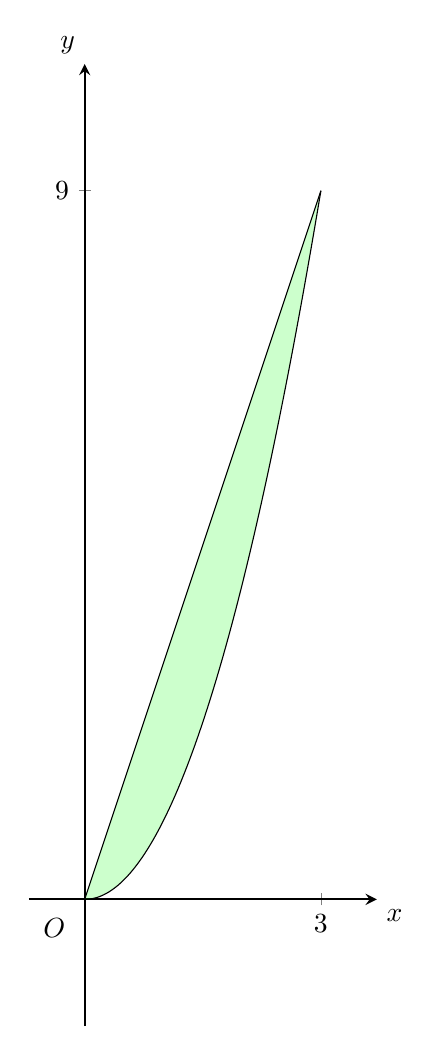
\begin{tikzpicture}
    \begin{axis}[standard,
            xtick={3},
            ytick={9},
            samples=100,
            xlabel={$x$},
            ylabel={$y$},
            xmin=-0.2,xmax=3.2,
            ymin=-0.2,ymax=9.2,
            x=1cm,
            y=1cm/1,
           ]
\node[anchor=center,label=south west:$O$] at (axis cs:0,0){};
\addplot[name path=F,domain={0:3}]{x^2};
\addplot[name path=G, domain={0:3}]{3*x};
\addplot[fill=green, fill opacity=0.2] fill between [of=F and G, soft clip={domain=0:3}];
    \end{axis}
    \end{tikzpicture}
}
\end{center}
The points of intersection are $(0,0)$ and $(3,9)$.

Remember: we want constants on the outside.

Therefore, we can do $x$'s on the outside and $y$'s on the inside to do
\begin{align*}
    V&=\int_0^3\int_{x^2}^{3x}x+4\,dy\,dx\\
    &=\int_0^3 \lrb{xy+4y}_{x^2}^{3x}\,dx\\
    &=\int_0^3 (3x^2+12x)-(x^3+4x^2)\,dx\\
    &=\int_0^3 -x^3-x^2+12x\,dx\\
    &=\lrb{-\frac{1}{4}x^4-\frac{1}{3}x^3+6x^2}_0^3\\
    &=\boxed{\frac{99}{4}}
\end{align*}

\textbf{Problem 6}

Find the volume of the solid in the first octant bounded by the coordinate planes, the plane $x=3$, and the parabolic cylinder $z=4-y^2$.

\Solution

The first octant is when $x,y,z\geq 0$. From $z=4-y^2$, we get $0=4-y^2$ which is just $y=\pm 2$ but remember: first octant!. We'll just keep the $y=2$.

Let's graph our boundaries. That is, graph $x=0$, $x=3$, $y=0$, $y=2$.
\begin{center}
\resizebox{3.5cm}{!}{
    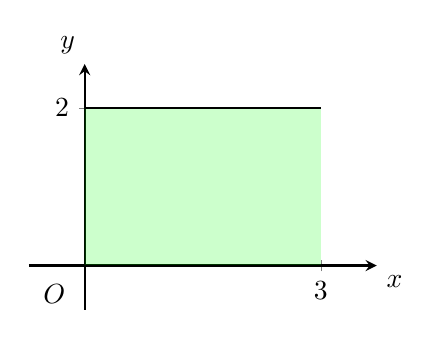
\begin{tikzpicture}
    \begin{axis}[standard,
            xtick={3},
            ytick={2},
            samples=100,
            xlabel={$x$},
            ylabel={$y$},
            xmin=-0.2,xmax=3.2,
            ymin=-0.2,ymax=2.2,
            x=1cm,
            y=1cm/1,
           ]
\node[anchor=center,label=south west:$O$] at (axis cs:0,0){};
\addplot[name path=F,domain={0:3}]{2};
\addplot[name path=G, domain={0:3}]{0};
\addplot[fill=green, fill opacity=0.2] fill between [of=F and G, soft clip={domain=0:3}];
    \end{axis}
    \end{tikzpicture}
}
\end{center}
Our double integral would be
\begin{align*}
    V&=\int_0^2\int_0^3 4-y^2\,dx\,dy\tag{easier to do $x$ then $y$}\\
    &=\int_0^2 \lrb{4x-xy^2}_0^3\,dy\\
    &=\int_0^2 12 -3y^2\,dy\\
    &=\lrb{12y-y^3}_0^2\\
    &=\boxed{16}
\end{align*}

You could have also done $\displaystyle \int_0^3 \int_0^2 4-y^2 \,dy\,dx$, but I think doing $x$ then $y$ is easier.

\textbf{Problem 7}

What region $R$ in the $xy$-plane minimizes the value of $\displaystyle \iint_R x^2+y^2-9\,dA$

\Solution

The function $z=x^2+y^2-9$ is a parabolid shifted $9$ units towards the $-z$ direction. 

Recall that the double integral is a \textit{signed} volume, so the bigger the negative volume is, the ``more minimal" the volume is.

We just want to find where $z=x^2+y^2-9\leq 0$ because we'll for sure get negative volume with negative $z$ values.

Writing the inequality out, we get
\begin{align*}
    x^2+y^2-9&\leq 0\\
    x^2+y^2&\leq 9
\end{align*}
\fbox{
    \parbox{0.9\linewidth}{
        The region $R$ where $x^2+y^2\leq9$ minimizes the value of $\displaystyle \iint_R x^2+y^2-9\,dA$. That is, the interior and boundary line of the circle $x^2+y^2=9$ is the region $R$ we're looking for.
    }
}

\textbf{Problem 8}

Calculate the average value of $f(x,y)=xy$ over the square $0\leq x\leq 1$, $0\leq y \leq 1$ and over the quarter-circle $x^2+y^2=1$ in the first quadrant.

\Solution
Recall that the average value of $f(x,y)$ is
\begin{align*}
    f(x,y)_{\text{avg}}=\frac{1}{A}\iint_R f(x,y)\,dA
\end{align*}
where $A$ is the area of the region $R$.

Over the square $0\leq x\leq 1$, $0\leq y \leq 1$, the area of the region would be a rectangle with length $1$ and width $1$
\begin{align*}
    f(x,y)_{\text{avg}}&=\frac{1}{(1)(1)}\int_0^1\int_0^1 xy\,dy\,dx\tag{order DOES NOT matter here}\\
    &=\int_0^1\lrb{\frac{1}{2}xy^2}_0^1\,dx\\
    &=\int_0^1 \frac{1}{2}x\,dx\\
    &=\lrb{\frac{1}{4}x^2}_0^1\\
    &=\boxed{\frac{1}{4}}
\end{align*}

Over the quarter-circle $x^2+y^2=1$ in the first quadrant, the area is $\displaystyle \frac{1}{4}\pi (1)^2=\frac{\pi}{4}$

We should also rewrite the circle equation into $y=\sqrt{1-x^2}$. We only keep the positive because we're in the first quadrant.

If you graphed the quarter circle, you'll notice that $x$ goes from $0$ to $1$.

Our average value is
\begin{align*}
    f(x,y)_{\text{avg}}=\frac{1}{\frac{\pi}{4}}\int_0^1\int_0^{\sqrt{1-x^2}} xy\,dy\,dx\\
    &=\frac{4}{\pi}\int_0^1\lrb{\frac{1}{2}xy^2}_0^{\sqrt{1-x^2}}\,dx\\
    &=\frac{4}{\pi}\int_0^1 \frac{1}{2}x(1-x^2)\,dx\\
    &=\frac{2}{\pi}\int_0^1 x-x^3\,dx\\
    &=\frac{2}{\pi}\lrb{\frac{1}{2}x^2-\frac{1}{4}x^4}_0^1\\
    &=\frac{2}{\pi}\lrp{\frac{1}{2}-\frac{1}{4}}\\
    &=\boxed{\frac{1}{2\pi}}
\end{align*}

\textbf{Problem 9}

Evaluate the (improper) double integral:

\textbf{(a)} $\displaystyle \int_1^{\infty}\int_{e^{-x}}^1\frac{1}{x^3y}\,dy\,dx$

\Solution
\begin{align*}
    \int_1^{\infty}\int_{e^{-x}}^1\frac{1}{x^3y}\,dy\,dx&=\int_1^\infty \lrb{\frac{1}{x^3}\ln\left|y\right|}_{e^{-x}}^1\,dx\\
    &=int_1^\infty (0)-\lrp{\frac{1}{x^3}(-x)}\,dx\\
    &=\int_1^\infty \frac{1}{x^2}\,dx\\
    &=\lim_{t\to\infty}\int_1^t \frac{1}{x^2}\,dx\\
    &=\lim_{t\to\infty}\lrb{-\frac{1}{x}}_1^t\\
    &=\lim_{t\to\infty} -\frac{1}{t}+\frac{1}{1}\\
    &=0+1\\
    &=\boxed{1}
\end{align*}
\textbf{(b)} $\displaystyle \int_{-\infty}^\infty\int_{-\infty}^\infty \frac{1}{(x^2+1)(y^2+1)}\,dx\,dy$

\Solution
\begin{align*}
    \int_{-\infty}^\infty\int_{-\infty}^\infty \frac{1}{(x^2+1)(y^2+1)}\,dx\,dy&=\int_{-\infty}^\infty \lim_{t\to -\infty}\int_{t}^0\frac{1}{(x^2+1)(y^2+1)}\,dx+\lim_{u\to\infty}\int_0^t\frac{1}{(x^2+1)(y^2+1)}\,dx\,dy\\
    &=\int_{-\infty}^\infty \lim_{t\to-\infty}\lrb{\frac{1}{y^2+1}\tan^{-1}x}_t^0+\lim_{u\to\infty}\lrb{\frac{1}{y^2+1}\tan^{-1}x}_0^u\,dy\\
    &=\int_{-\infty}^\infty \lim_{t\to\infty}\lrp{0-\frac{1}{y^2+1}\tan^{-1}t}+\lim_{u\to\infty}\lrp{\frac{1}{y^2+1}\tan^{-1}u-0}\,dy\\
    &=\int_{-\infty}^\infty \lrp{0+\frac{1}{y^2+1}\frac{\pi}{2}}+\lrp{\frac{1}{y^2+1}\frac{\pi}{2}-0}\,dy\\
    &=\int_{-\infty}^\infty \frac{2\pi}{2(y^2+1)}\,dy\\
    &=\pi\int_{-\infty}^\infty \frac{1}{y^2+1}\,dy\\
    &=\pi\Big(\lim_{t\to-\infty}\int_t^0\frac{1}{y^2+1}+\lim_{u\to\infty}\int_0^u\frac{1}{y^2+1}\,dy\Big)\\
    &=\pi\lrp{\lim_{t\to-\infty}\lrb{\tan^{-1}y}_t^0+\lim_{u\to\infty}\lrb{\tan^{-1}y}_0^u}\\
    &=\pi\lrp{\frac{\pi}{2}+\frac{\pi}{2}}\tag{we did this earlier}\\
    &=\pi\lrp{\pi}\\
    &=\boxed{\pi^2}
\end{align*}
\textbf{Problem 10}

Evaluate the integral $\displaystyle \int_0^2\tan^{-1}\pi x -\tan^{-1}x\,dx$

\Solution

As the hint says, let's write this as a double integral.
\begin{align*}
    \int_0^2\tan^{-1}\pi x -\tan^{-1}x\,dx&=\int_0^2\lrb{\tan^{-1}y}_{x}^{\pi x}\,dx\\
    &=\int_0^2\int_x^{\pi x} \frac{1}{(y^2+1)}\,dy\,dx\tag{what's the derivative of $\tan^{-1}y$?}
\end{align*}
To change the order of integration, we need to know our boundaries. That is, graph $x=0$, $x=2$, $y=x$, 

We'll also need to break up the region along the line $y=2$ if we want to have $y$ on the outside (as it goes from $0\leq y \leq 2\pi$). Our integral now becomes
\begin{align*}
    \int_0^2\int_x^{\pi x} \frac{1}{(y^2+1)}\,dy\,dx&=\int_0^2 \int_{\frac{y}{\pi}}^y\frac{1}{y^2+1}\,dx\,dy+\int_2^{2\pi}\int_{\frac{y}{\pi}}^2\frac{1}{y^2+1}\,dx\,dy\\
    &=\int_0^2\lrb{\frac{1}{y^2+1}x}_{y/\pi}^y\,dy+\int_2^{2\pi}\lrb{\frac{1}{y^2+1}x}_{y/\pi}^2\\
    &=\int_0^2 \frac{1}{y^2+1}\lrp{y-\frac{y}{\pi}}\,dy+\int_2^{2\pi}\frac{1}{y^2+1}\lrp{2-\frac{y}{\pi}}\,dy\\
    &=\lrp{1-\frac{1}{\pi}}\int_0^2\frac{y}{y^2+1}\,dy+\int_2^{2\pi} \frac{2}{y^2+1}-\frac{y}{\pi(y^2+1)}\,dy\\
    &=\lrp{\frac{\pi -1}{2\pi}}\lrb{\ln(1+y^2)}_0^2+\lrb{2\tan^{-1}y-\frac{1}{2\pi}\ln(1+y^2)}_2^{2\pi}\\
    &=\lrp{\frac{\pi-1}{2\pi}}\ln 5 + \lrp{2\tan^{-1}2\pi -\frac{1}{2\pi}\ln(1+4\pi^2)}-\lrp{2\tan^{-1}2-\frac{1}{2\pi}\ln(5)}\\
    &=\lrp{\frac{(\pi-1)+1}{2\pi}}\ln 5 + 2\tan^{-1}2\pi -\frac{1}{2\pi}\ln (1+4\pi^2)-2\tan^{-1}2\\
    &=\boxed{\frac{1}{2}\ln 5 + 2\tan^{-1}2\pi -\frac{1}{2\pi}\ln (1+4\pi^2)-2\tan^{-1}2}
\end{align*}
\end{document}